\documentclass[12pt]{letter}\usepackage[letterpaper,margin=0.65in]{geometry}\usepackage{textcomp}\usepackage{graphicx}\usepackage[rflt]{floatflt}\pagenumbering{gobble}\begin{document}\begin{floatingfigure}{0.15\textwidth}\raisebox{0pt}[0pt][0pt]{\raisebox{-2.5cm}{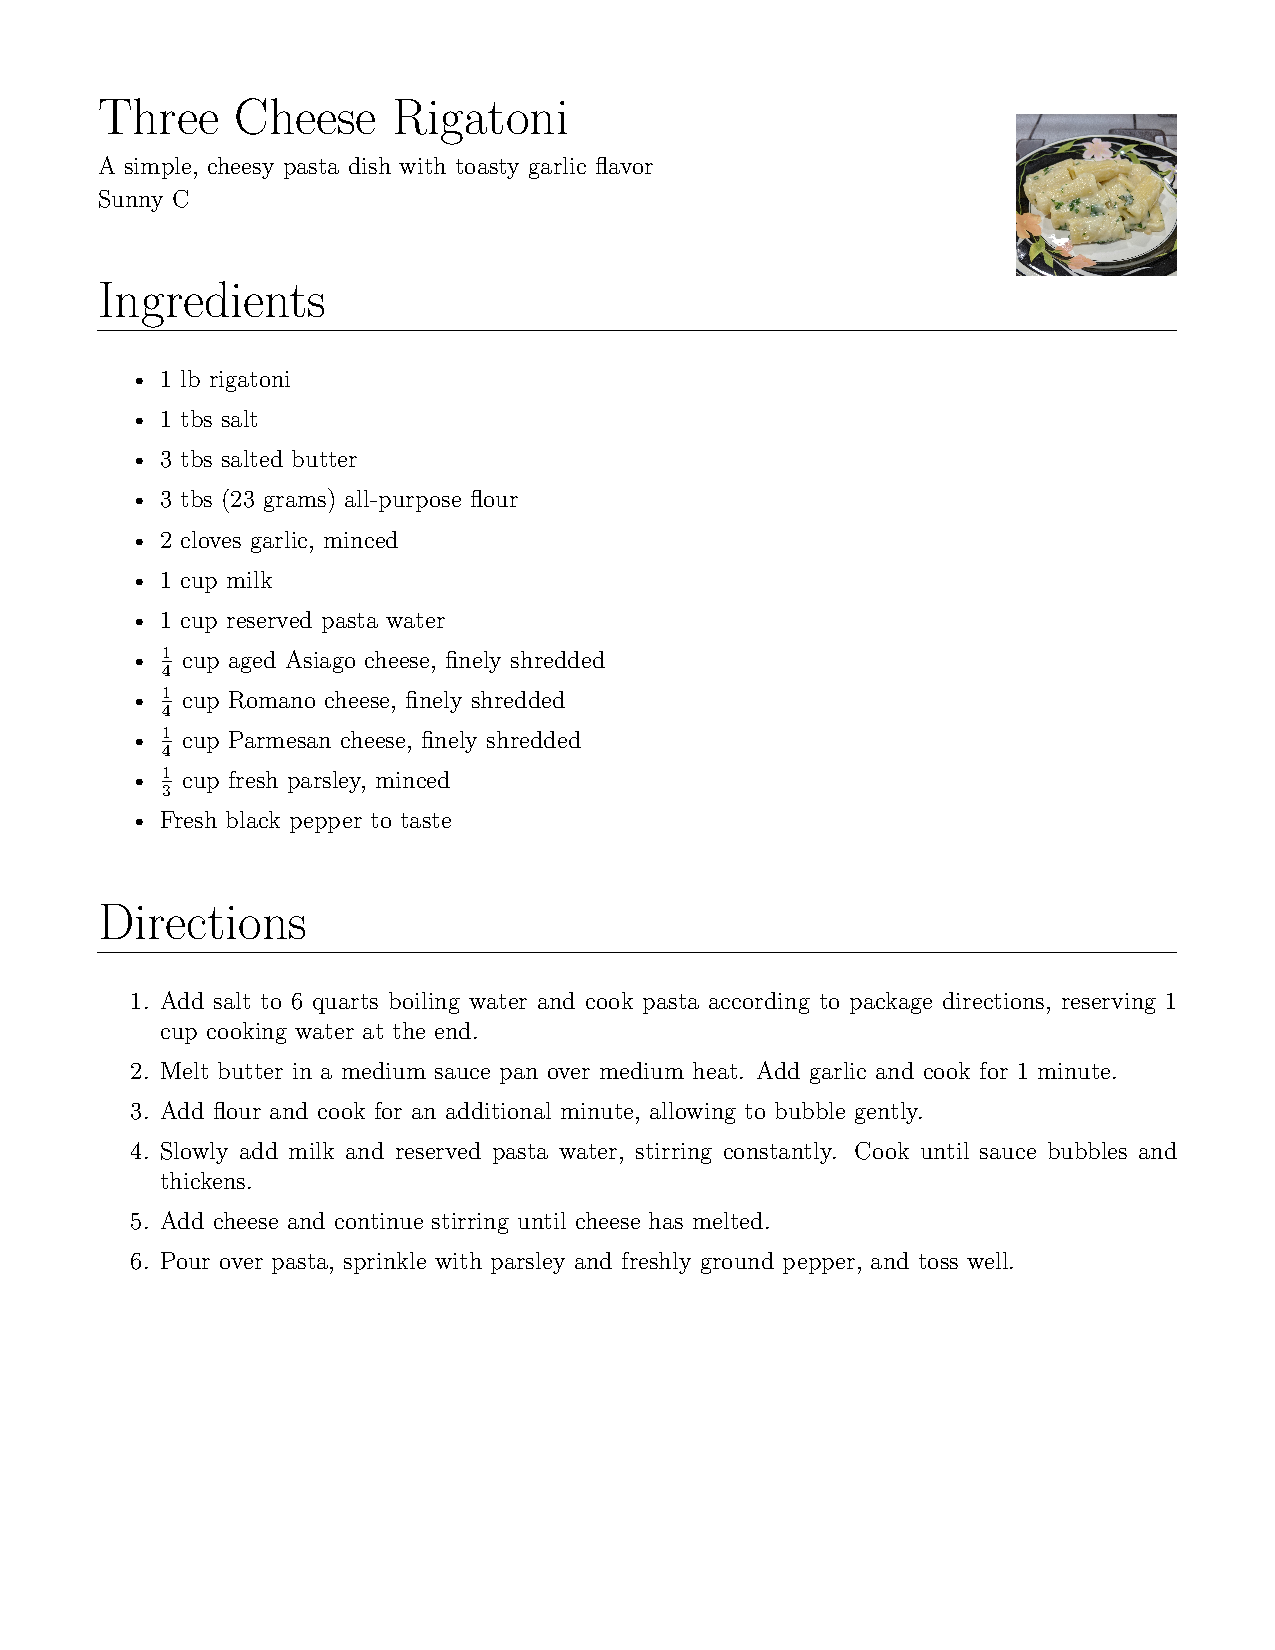
\includegraphics[width=0.15\textwidth]{three-cheese-rigatoni}}}\end{floatingfigure}\begin{huge}Three Cheese Rigatoni\end{huge}\newline\vspace{-2.5mm}\newline\renewcommand{\arraystretch}{1.1}\begin{tabular*}{\textwidth}{@{\extracolsep{\fill}}lr}A simple, cheesy pasta dish with toasty garlic flavor\\Sunny C\end{tabular*}\newline\vspace{10mm}\newline\begin{huge}Ingredients\end{huge}\\\rule[2.8mm]{\textwidth}{.1pt}\vspace{-3mm}\begin{itemize}\item 1 lb rigatoni\item 1 tbs salt\item 3 tbs salted butter\item 3 tbs all-purpose flour\item 2 cloves garlic, minced\item 1 cup milk\item 1 cup reserved pasta water\item $\frac{1}{4}$ cup aged Asiago cheese, finely shredded\item $\frac{1}{4}$ cup Romano cheese, finely shredded\item $\frac{1}{4}$ cup Parmesan cheese, finely shredded\item $\frac{1}{3}$ cup fresh parsley, minced\item Fresh black pepper to taste\end{itemize}\vspace{7mm}\begin{huge}Directions\end{huge}\\\rule[2.8mm]{\textwidth}{.1pt}\vspace{-3mm}\begin{enumerate}\item Add salt to 6 quarts boiling water and cook pasta according to package directions, reserving 1 cup cooking water at the end.\item Melt butter in a medium sauce pan over medium heat. Add garlic and cook for 1 minute.\item Add flour and cook for an additional minute, allowing to bubble gently.\item Slowly add milk and reserved pasta water, stirring constantly. Cook until sauce bubbles and thickens.\item Add cheese and continue stirring until cheese has melted.\item Pour over pasta, sprinkle with parsley and freshly ground pepper, and toss well.\end{enumerate}\end{document}